\documentclass[11pt]{article}

\usepackage[utf8]{inputenc}
\usepackage[english]{babel}
\usepackage[english]{isodate}
\usepackage[parfill]{parskip}

\usepackage{graphicx}
%%
% Just some sample text
\usepackage{lipsum}
\usepackage{tabularx}
\usepackage{xcolor} % for colour
\usepackage{colortbl}
%\usepackage{multirow}
\usepackage{lettrine}

\usepackage{amsmath}
\usepackage{mathtools}
\usepackage{amssymb}
\usepackage{nccmath}
\usepackage{relsize}
\usepackage{biblatex} %Imports biblatex package

\usepackage[colorlinks=true,allcolors=black]{hyperref}

\addbibresource{refs.bib} %Import the bibliography file

\usepackage{geometry}
 \geometry{
	a4paper,
	total={170mm,257mm},
	left=20mm,
	top=20mm,
}



\title{AC-DC power flow modeling technical note}

\author{Santiago Pe\~nate Vera and Josep Fanals i Batllori}
\begin{document}
	
	\maketitle
	
%% -----------------------------------------------------------------------------------------------------------------
%% COUPLED CONVERTER 
%% -----------------------------------------------------------------------------------------------------------------
	
	\section{Converter coupled AC-DC modeling}
	
	Converter coupled modeling was introduced in the PhD thesis of Abraham Álvarez (Universal branch model for the solution of optimal power flows in hybrid AC/DC grids). In this modeling framework the converters are treated as a regular branch with a shunt susceptance ($b_{eq}$) that is used to make zero the reactive power at the DC side (the from side) of the branch.
	
	\begin{figure}[h!]
		\centering
		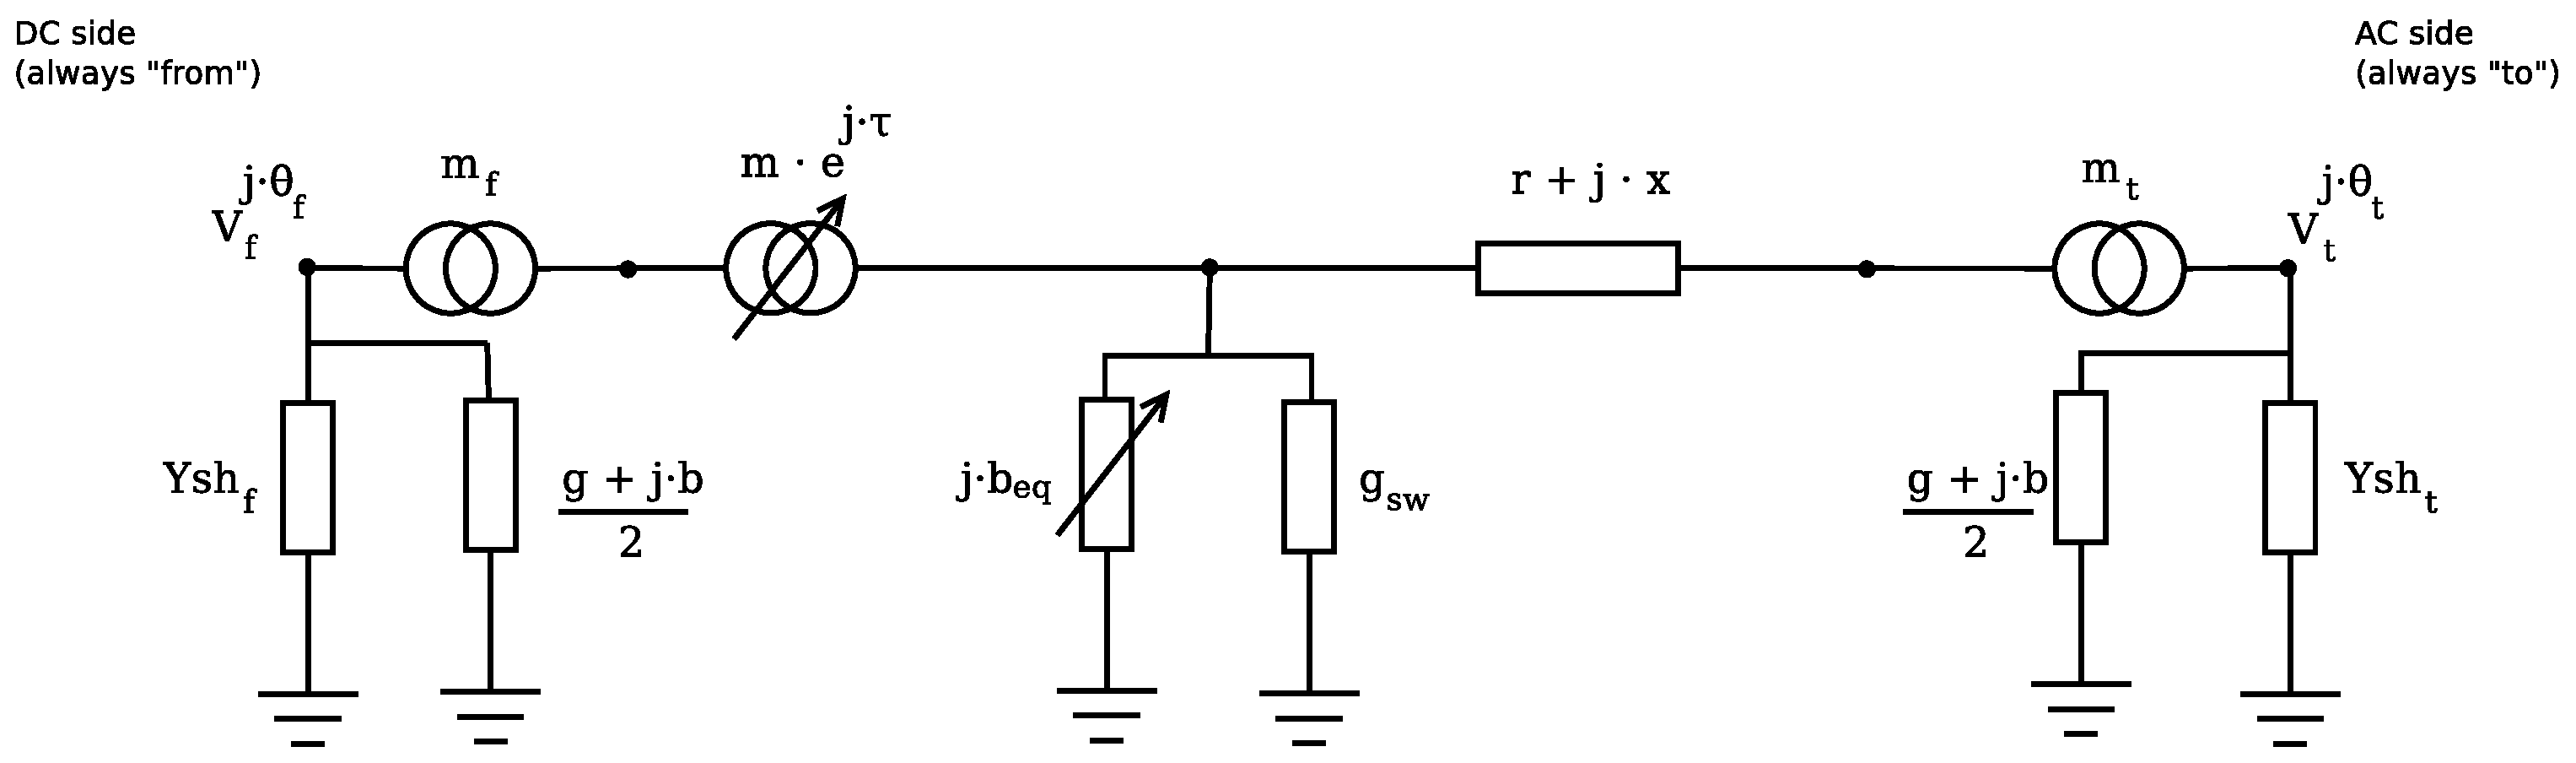
\includegraphics[width=0.8\linewidth]{fubm.eps}
		\caption{Full Unified Branch Model.}
		\label{fig:fubm}
	\end{figure}
	
	
	The power flow linearization formulation is:
	
	\begin{equation}
		\begin{bmatrix}
			\frac{\partial P}{\partial \theta} & \frac{\partial P}{\partial Vm} & \frac{\partial P}{\partial b_{eq}} & \frac{\partial P}{\partial m} & \frac{\partial P}{\partial \tau} \\
			\frac{\partial Q}{\partial \theta} & \frac{\partial Q}{\partial Vm} & \frac{\partial Q}{\partial b_{eq}} & \frac{\partial Q}{\partial m} & \frac{\partial Q}{\partial \tau} \\
			\frac{\partial Q_f}{\partial \theta} & \frac{\partial Q_f}{\partial Vm} & \frac{\partial Q_f}{\partial b_{eq}} & \frac{\partial Q_f}{\partial m} & \frac{\partial Q_f}{\partial \tau} \\
			\frac{\partial Q_t}{\partial \theta} & \frac{\partial Q_t}{\partial Vm} & \frac{\partial Q_t}{\partial b_{eq}} & \frac{\partial Q_t}{\partial m} & \frac{\partial Q_t}{\partial \tau} \\
			\frac{\partial P_f}{\partial \theta} & \frac{\partial P_f}{\partial Vm} & \frac{\partial P_f}{\partial b_{eq}} & \frac{\partial P_f}{\partial m} & \frac{\partial P_f}{\partial \tau} \\
			\frac{-\partial P_f}{\partial \theta} & \frac{\partial P_{fdp}}{\partial Vm} & \frac{-\partial P_{f}}{\partial b_{eq}} & \frac{-\partial P_{f}}{\partial m} & \frac{-\partial P_{f}}{\partial \tau} \\
		\end{bmatrix}	
		\times 
		\begin{bmatrix*}[l]
			\Delta \theta  \quad \quad \ \forall \ i_{pv} \cup i_{pq}  \\
			\Delta Vm  \quad   \forall \ i_{pq}  \\
			\Delta b_{eq}  \quad \ \ \forall  \ k_{zero}^{b_{eq}} \cup k_{V_f}^{b_{eq}}  \\	
			\Delta m  \quad \quad \forall  \ k_{Q_f}^m \cup k_{Q_t}^m \cup k_{V_t}^m  \\
			\Delta \tau  \quad \quad \ \forall \ k_{P_f}^\tau \cup k_{P_f}^{dp}
		\end{bmatrix*}
		= 
		\begin{bmatrix*}[l]
			\Delta P \quad \ \ \forall \ i_{pv} \cup i_{pq} \\
			\Delta Q \quad \ \ \forall \ i_{pq} \cup i_{V_f}^{b_{eq}} \cup i_{V_t}^m  \\
			\Delta Q_f \quad \forall \ k_{Q_f}^m \cup k_{zero}^{b_{eq}} \\
			\Delta Q_t \quad \ \forall \ k_{Q_t}^m  \\
			\Delta P_f \quad \ \forall \ k_{P_f}^\tau  \\
			\Delta P_{dp} \quad \forall \ k_{P_f}^{dp}
		\end{bmatrix*}
	\end{equation}

	
	
	The droop power residual is:
	
	\begin{equation}
		\Delta P_{dp} = -P_f^{calc} - (P_f^{esp} + K_{dp} \cdot ( Vm_{f} - Vm_{f}^{esp} ))
	\end{equation}
	
	
	Note that when formulating the problem, we have two bus-related unknowns ($\Delta \theta$, $\Delta Vm$) and two equations ($\Delta P$, $\Delta Q$) and for these, variations occur respecting the two-unknown, two-equations restriction. For the branches we have three unknowns ($\Delta b_{eq}$, $\Delta m$, $\Delta \tau$) and equations to match. So for the branches we must respect the relation of the branch unknowns to the branch equations. That is done with the indexing. Hence, the indices are very relevant in this formulation:
	
	\begin{itemize}
		
		\item $i_{pv}$: Indices of the PV buses.
		\item $i_{pq}$: Indices of the PQ buses.
		\item $k_{zero}^{b_{eq}}$: indices of the branches (converters) making $Q_f=0$ with $b_{eq}$.
		\item $k_{V_f}^{b_{eq}}$: indices of the branches controlling $V_f$ with $b_{eq}$.
		\item $i_{V_f}^{b_{eq}}$: indices of the \textit{from} buses of branches controlling $V_f$ with $b_{eq}$.
		
		\item $k_{Q_f}^m$: indices of the branches controlling $Q_f$ with $m$.
		\item $k_{Q_t}^m$: indices of the branches controlling $Q_t$ with $m$.
		\item $k_{V_t}^m$: indices of the branches controlling $V_t$ with $m$.
		
		\item $i_{V_t}^m$: indices of the \textit{to} buses of the branches controlling $V_t$ with $m$.
		
		\item $k_{P_f}^\tau$: indices of the branches controlling $P_f$ with $\tau$.
		\item $k_{P_f}^{dp}$: indices of the branches with voltage droop control.
	\end{itemize}
	
	Observe that $i$ is used for bus indexing with the bus-related magnitudes ($\theta$, $Vm$, $P$ and $Q$).
	$k$ is used for branch related indexing with the branch-related magnitudes ($b_{eq}$, $m$, $\tau$, $P_f$, $Q_f$ and $Q_t$)
	
	\subsection{Example}
	
	\begin{figure}[h!]
		\centering
		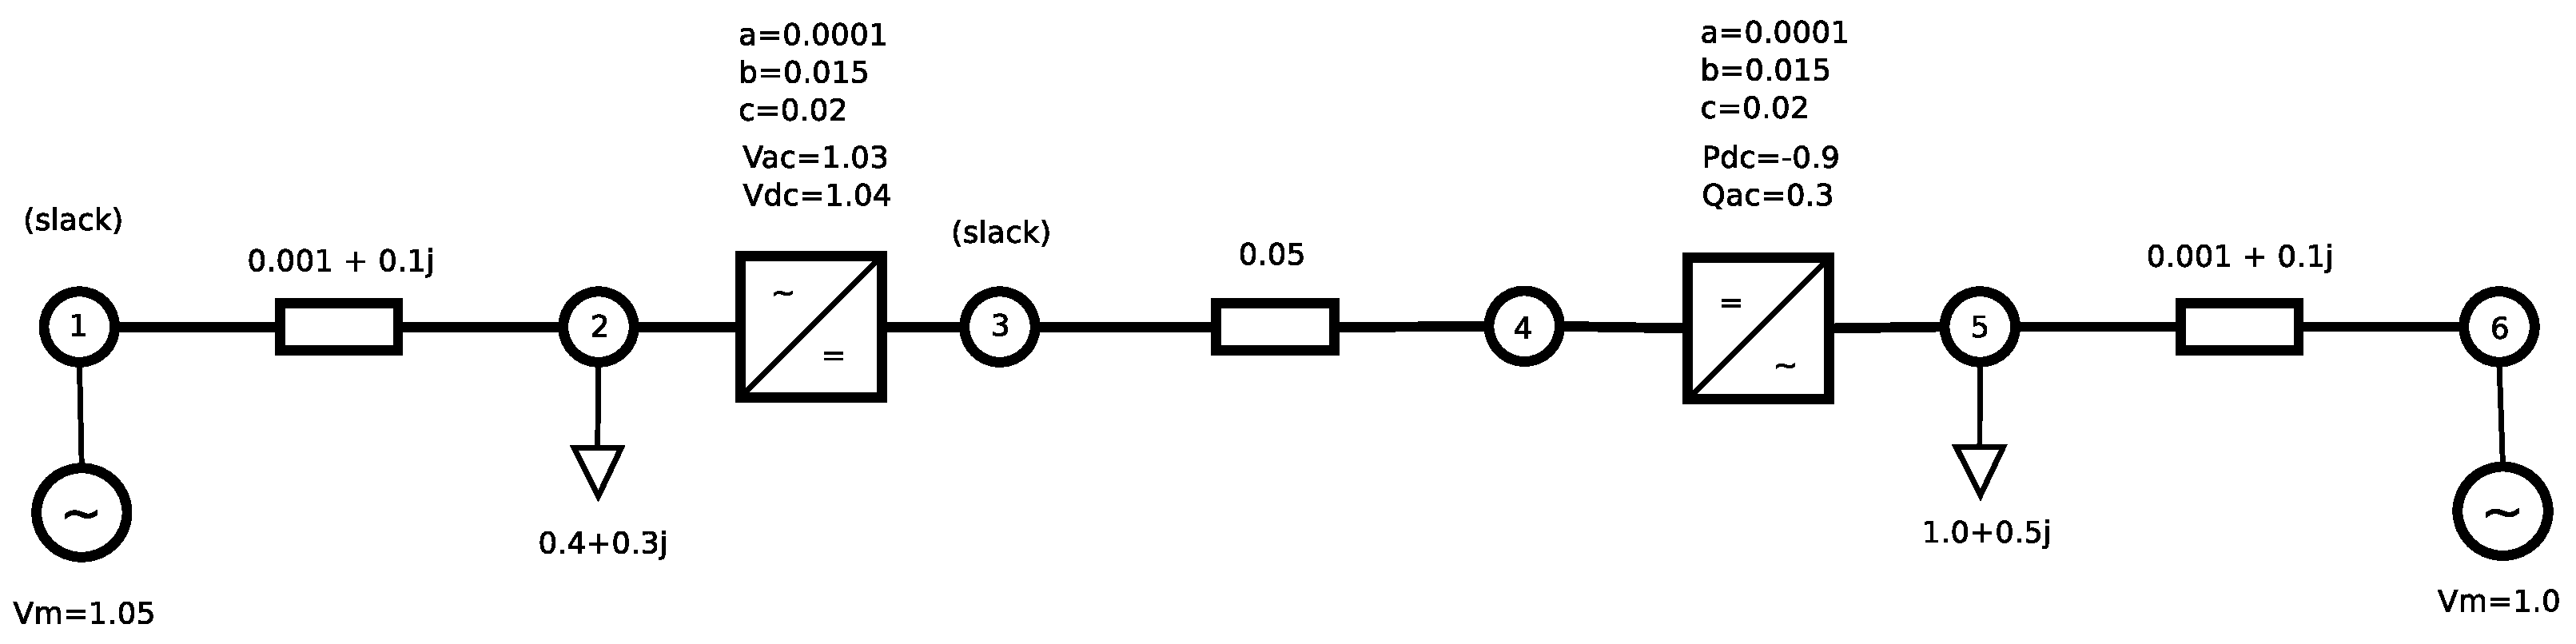
\includegraphics[width=1.0\linewidth]{acdc_6bus_diagram_fubm}
		\caption{Coupled converter model example grid.}
		\label{fig:acdc6busdiagram_fubm}
	\end{figure}

	

%% -----------------------------------------------------------------------------------------------------------------
%% DECOUPLED CONVERTER 
%% -----------------------------------------------------------------------------------------------------------------
	\newpage
	\section{Converter decoupled AC-DC modeling}
	
	The converter is a decoupled branch in the sense that the \textit{from} and \textit{to} sides are not galvanically connected in the model. The converter is \textit{hollow}. Hence, the coupling needs to be done via equations in the jacobian matrix since the coupling cannot be done in the admittance matrix.
	
	\begin{table}[h!]
	\begin{tabular}{cc} % The table has 2 columns, both centered (cc)
		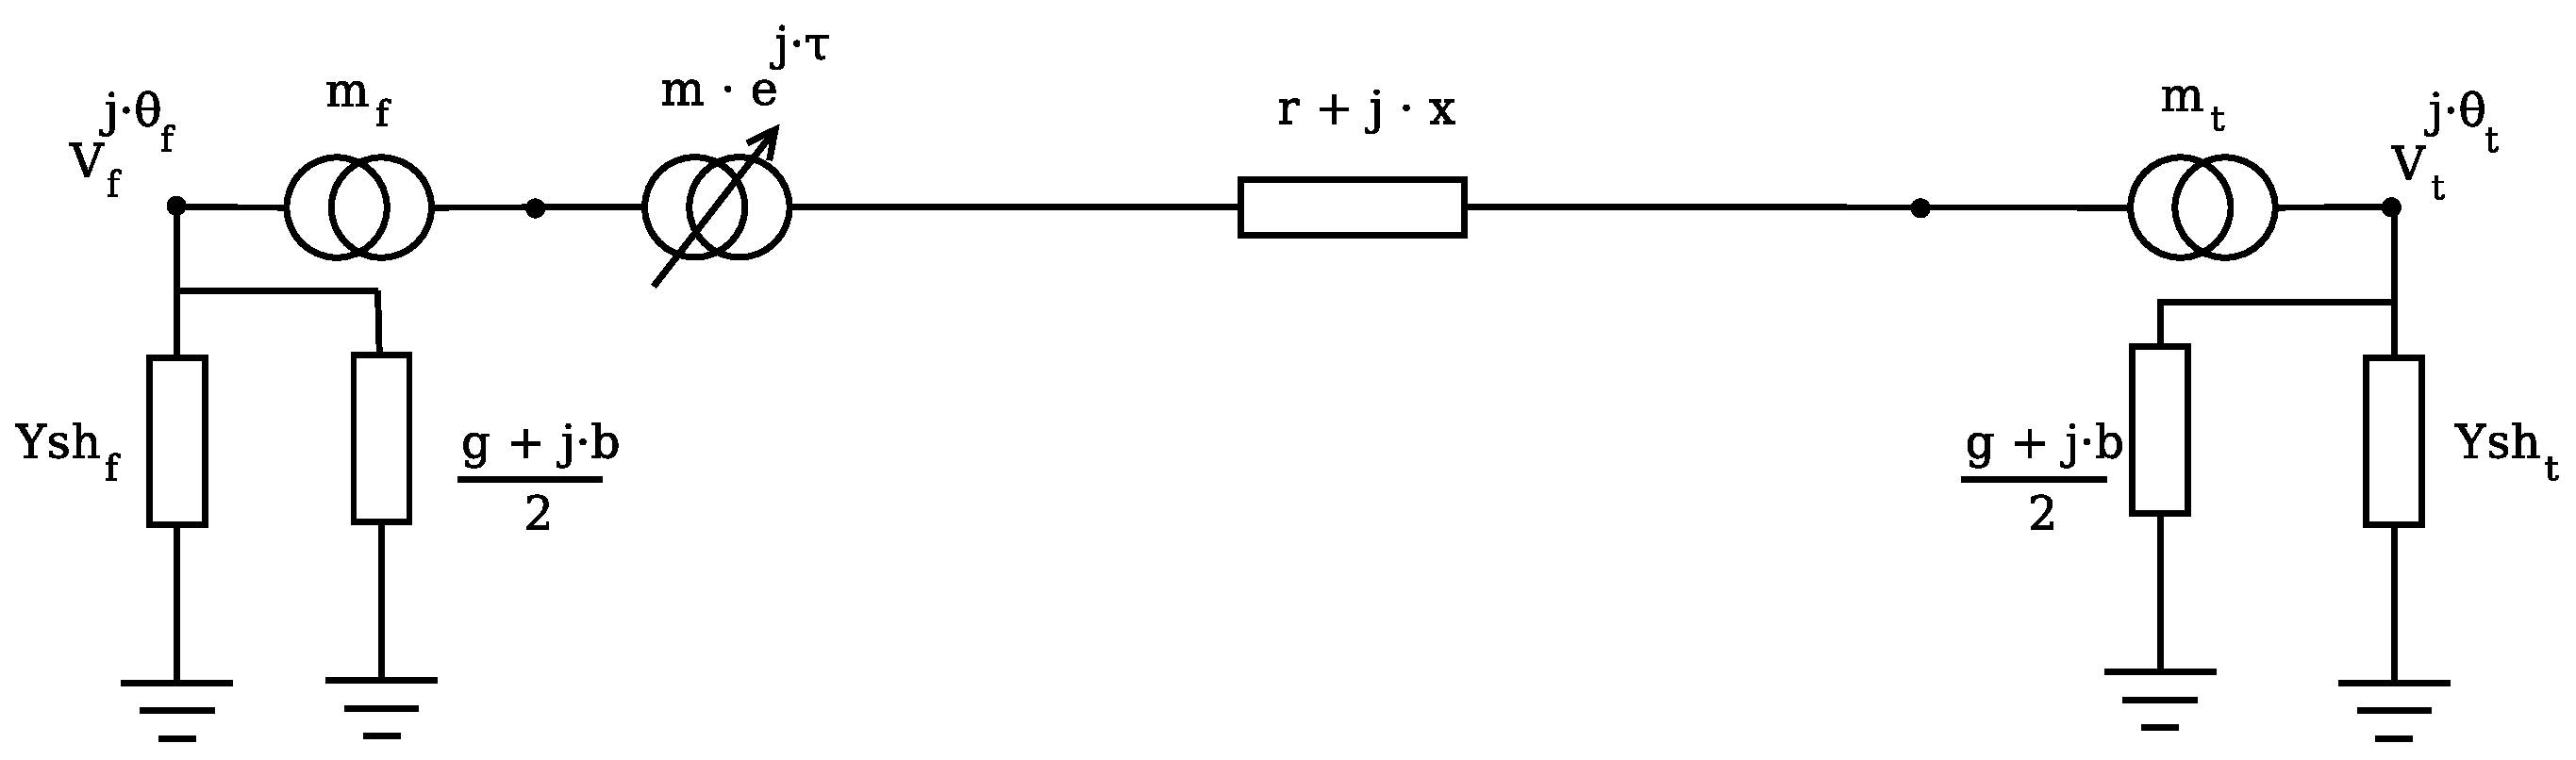
\includegraphics[width=0.65\linewidth]{branch.eps} &
		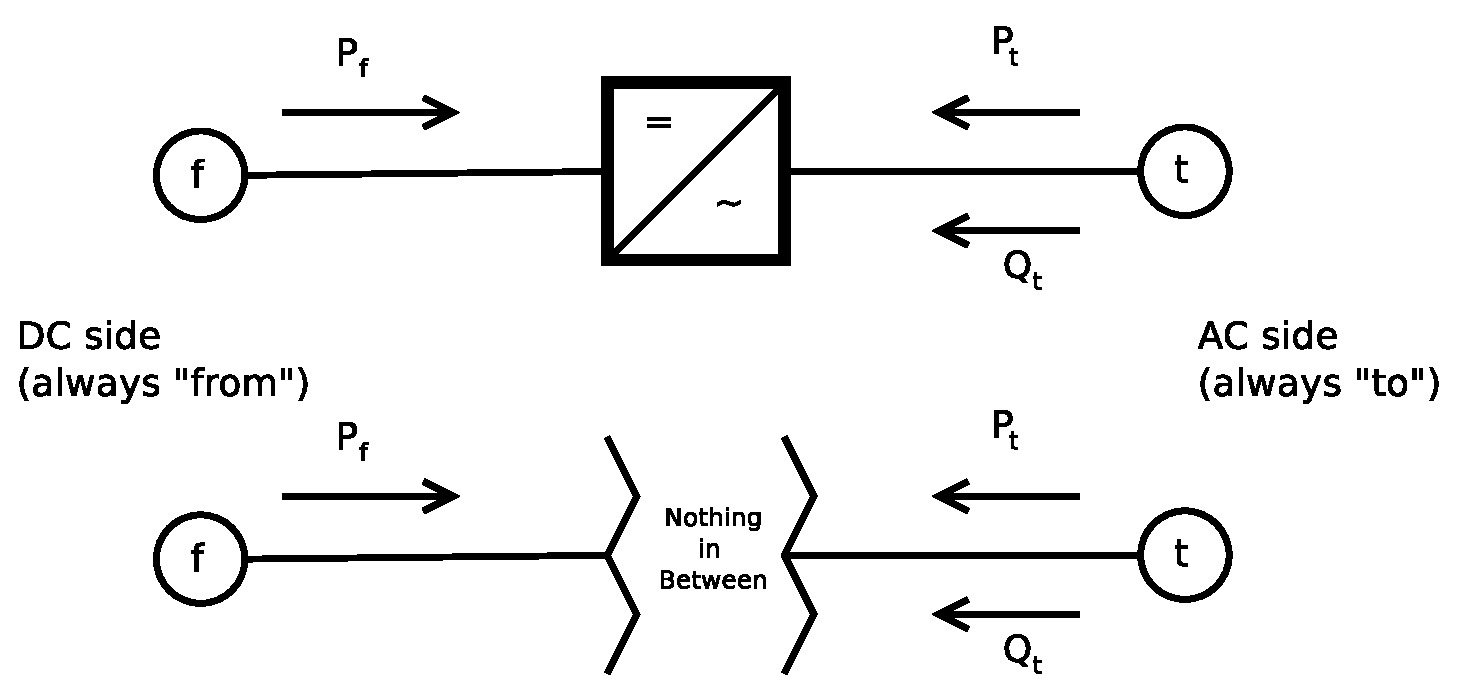
\includegraphics[width=0.35\linewidth]{decoupled_converter_model.eps} \\
	\end{tabular}
	\caption{General branch on the left. Decoupled converter model on the right}
	\label{table:branch_and_converter}
	\end{table}
	
	The power flow linearization formulation is:
	
	\begin{equation}
		\label{eq:acdc_syst}
		\begin{bmatrix}
			\frac{\partial P}{\partial \theta} & \frac{\partial P}{\partial V_m} & \frac{\partial P}{\partial P_f^{conv}} & \frac{\partial P}{\partial P_t^{conv}} & \frac{\partial P}{\partial Q_t^{conv}}\\
			\frac{\partial Q}{\partial \theta} & \frac{\partial Q}{\partial V_m} & \frac{\partial Q}{\partial P_f^{conv}} & \frac{\partial Q}{\partial P_t^{conv}} & \frac{\partial Q}{\partial Q_t^{conv}}\\
			\frac{\partial P_{conv}^{conv}}{\partial \theta} & \frac{\partial P_{eq}^{conv}}{\partial V_m} & \frac{\partial P_{eq}^{conv}}{\partial P_f^{conv}} & \frac{\partial P_{eq}^{conv}}{\partial P_t^{conv}} & \frac{\partial P_{eq}^{conv}}{\partial Q_t^{conv}}\\
		\end{bmatrix}	
		\times 
		\begin{bmatrix*}[l]
			\Delta \theta  \quad \forall \ i_{pv} \cup i_{pq}   \\
			\Delta V_m     \quad \forall \ i_{pq}  \\
			\Delta P_f^{conv}     \quad \forall \ k_{conv} \\
			\Delta P_t^{conv}     \quad \forall \ k_{conv} \\
			\Delta Q_t^{conv}     \quad \forall \ k_{conv}
		\end{bmatrix*}
		= 
		\begin{bmatrix*}[l]
			\Delta P \quad \ \ \forall \ i_{pv} \cup i_{pq} \\
			\Delta Q \quad \ \ \forall \ i_{pq}  \\
			\Delta P_{eq}^{conv} \quad \forall \ k_{conv} 
		\end{bmatrix*}
	\end{equation}

\begin{itemize}
	
	\item $i_{pv}$: Indices of the PV buses.
	\item $i_{pq}$: Indices of the PQ buses.
	\item $k_{conv}$: Indices of the converters.
\end{itemize}
	
	
	Active power nodal balance:
	\begin{equation}
		\Delta P = P^{calc} - P^{esp}
	\end{equation}
	
	
	Reactive power nodal balance:
	\begin{equation}
		\Delta Q = Q^{calc} - Q^{esp}
	\end{equation}
	
		
	Converter power balance:
	
	\begin{equation}
		\Delta P_{eq}^{conv} = P_f^{conv} + P_t^{conv} - P_{loss}^{conv}
	\end{equation}
	
	In this equation $P_f^{conv}$ and $P_t^{conv}$ are variables to be found iteratively, and are not the same as the regular branches power flow ($P_f$, $P_t$) since these variables are introduced to couple the linear system and avoid singularities.
	
	\subsection{Example}
	
	
	\begin{figure}[h!]
		\centering
		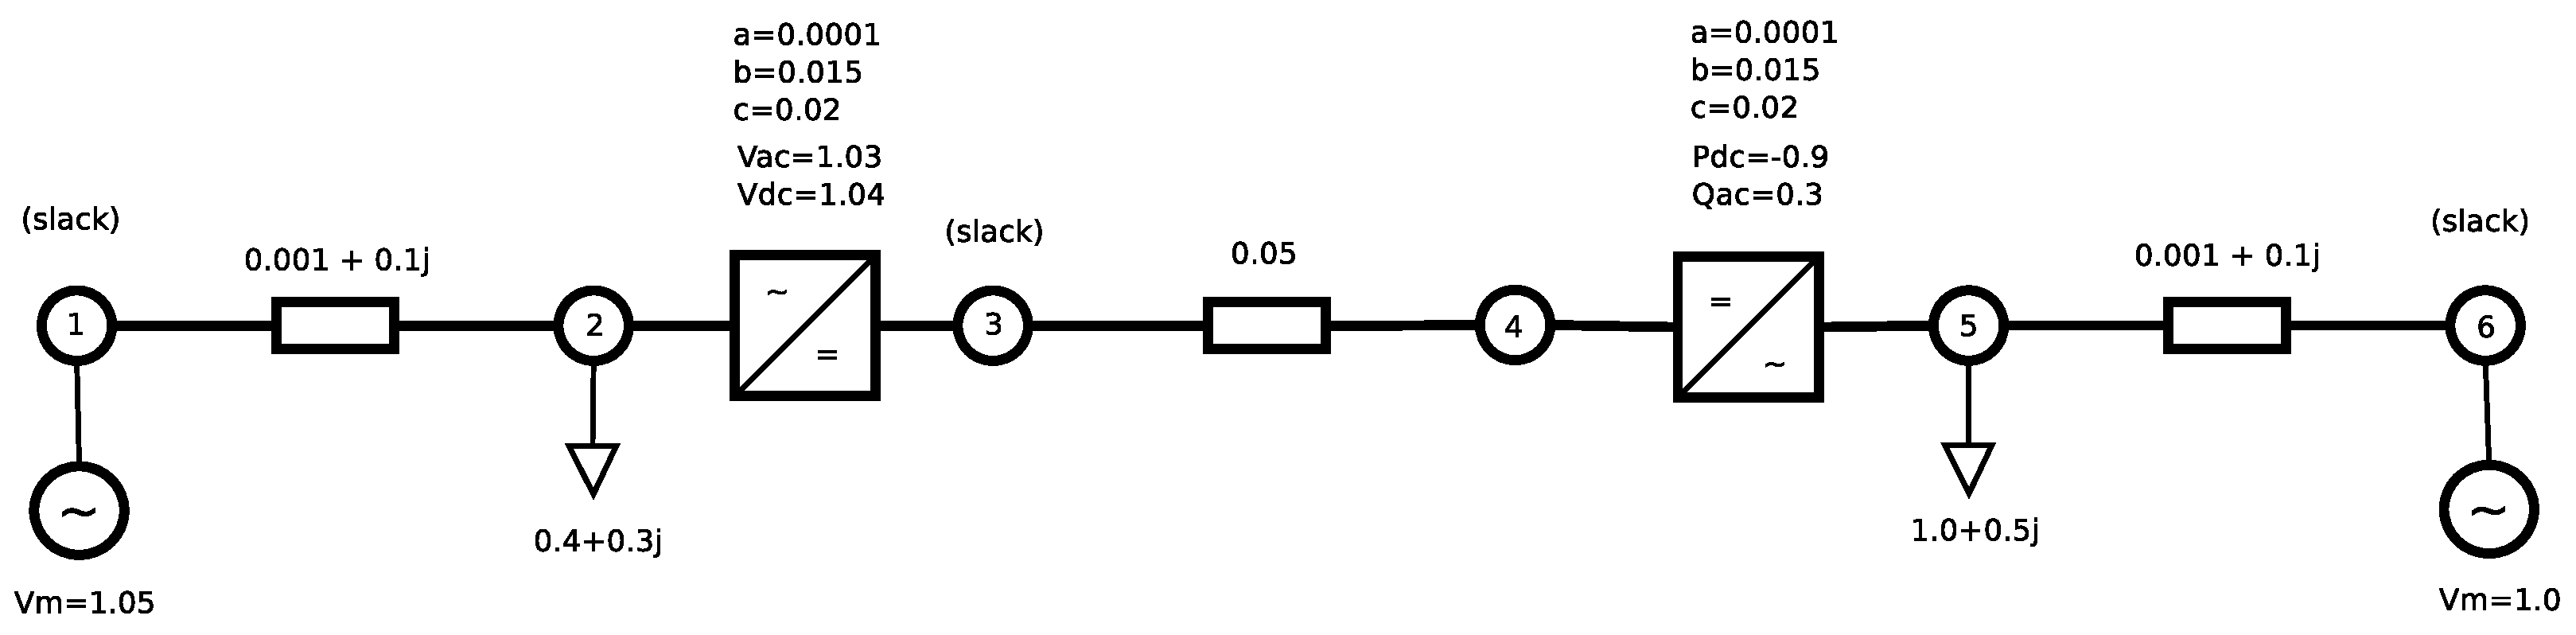
\includegraphics[width=1.0\linewidth]{acdc_6bus_diagram}
		\caption{Decoupled converter model example grid.}
		\label{fig:acdc6busdiagram}
	\end{figure}
	

	\newpage

	\section{Control mapping}
	It is assumed that each converter controls two magnitudes. Then, the control modes are the ones indicated in Table~\ref{table:contr_vsc}, as described in~\cite{alvarez2021universal}. The AC and DC sides of each control mode are classified into grid-forming (GFM) or grid-following (GFL) following the principles depicted in~\cite{gomis2020principles}.

	\begin{table}[!htb]\centering
		\caption{Control modes and types of VSCs with the corresponding constraints.}
		\begin{tabular}{ccccc}
			\hline
			\textbf{Control mode} & \textbf{DC Variable} & \textbf{AC Variable} & \textbf{AC Type} & \textbf{DC Type} \\
			\hline
			1 & - & $\theta$, $V_t$ & GFM & GFL \\
			2 & $P_f$ & $Q_t$ & GFL & GFL \\
			3 & $P_f$ & $V_t$ & GFL & GFL \\
			4 & $V_f$ & $Q_t$ & GFL & GFM \\
			5 & $V_f$ & $V_t$ & GFL & GFM \\
			6 & $V_f$ droop & $Q_t$ & GFL & GFM \\
			7 & $V_f$ droop & $V_t$ & GFL & GFM \\
			\hline
		\end{tabular}
		\label{table:contr_vsc}
	\end{table}

	There are only 2 rules to be followed when setting the control modes of VSCs:
	\begin{enumerate}
		\item Each AC grid has to have only 1 slack bus where $\theta$ and $V$ are set.
		\item Each DC grid has to have only 1 slack bus where $V$ is set.
	\end{enumerate}
	The next step is to merge the controls in Table~\ref{table:contr_vsc} with the system of equations~\eqref{eq:acdc_syst}. Table~\ref{table:vsc_map} identifies the map between the known and unknown variables and the controls.

	\begin{table}[!htb]\centering
		\caption{Control modes and types of VSCs with the corresponding constraints.}
		\begin{tabular}{ccccccc}
			\hline
			\textbf{Mode} & \textbf{Bus from} & \textbf{Bus to} & \textbf{Known} & \textbf{Known} & \textbf{Unknown} & \textbf{Unknown} \\
			\textbf{} & \textbf{DC} & \textbf{AC} & \textbf{DC} & \textbf{AC} & \textbf{DC} & \textbf{AC} \\
			\hline
			1 & $P$ & Slack & - & $\theta$, $V_t$ & $V_f$, $P_f$ & $P_t$, $Q_t$ \\
			2 & $P$ & $PQ$ & $P_f$ & $Q_t$ & $V_f$ & $\theta$, $V_t$, $P_t$ \\
			3 & $P$ & $PV$ & $P_f$ & $V_t$ & $V_f$ & $\theta$, $P_t$, $Q_t$ \\
			4 & $V$ & $PQ$ & $V_f$ & $Q_t$ & $P_f$ & $\theta$, $V_t$, $P_t$ \\
			5 & $V$ & $PV$ & $V_f$ & $V_t$ & $P_f$ & $\theta$, $P_t$, $Q_t$ \\
			6 & $V$ & $PQ$ & $V_f$ droop & $Q_t$ & $P_f$ & $\theta$, $V_t$, $P_t$ \\
			7 & $V$ & $PV$ & $V_f$ droop & $V_t$ & $P_f$ & $\theta$, $P_t$, $Q_t$ \\
			\hline
		\end{tabular}
		\label{table:vsc_map}
	\end{table}



	
	\section{Bibliography}
	\printbibliography
	
\end{document}